\documentclass[french,12pt]{article}
\usepackage[T1]{fontenc}
\usepackage[utf8]{inputenc}
\usepackage{kpfonts}
\usepackage{babel}
\usepackage{microtype}
\usepackage{graphicx}
\usepackage{geometry}
\usepackage{hyperref}
\usepackage{acronym}
\usepackage[lofdepth,lotdepth]{subfig}
\usepackage[backend=biber,style=trad-alpha]{biblatex} 

\bibliography{document.bib} % or
\geometry{hmargin=3cm,vmargin=2cm}

\title{État de l'art - spatial}

\acrodef{ENP}{Expressive Notation Package}
\acrodef{GPU}{Graphics Processing Unit}
\acrodef{DBAP}{Distance-Based Amplitude Panning}
\acrodef{VBAP}{Vector Base Amplitude Panning}
\acrodef{WFS}{Wave-Field Synthesis}
\acrodef{GIS}{Geographic Information Service}
\acrodef{WIMP}{Windows, Icons, Menus and Pointing device}
\begin{document}
\maketitle
\tableofcontents

\section{Introduction}
Ce document vise à présenter un état de l'art des pratiques impliquant la manipulation de 
données spatiales dans un cadre artistique, interactif et muséographique.

Nous présentons notamment les besoins des concepteurs, ainsi que les diverses solutions qui 
peuvent y être apportées, que ce soit par la conception de logiciels dédiés ou bien 
par des modélisations formelles des notions d'espace.
 
\begin{itemize}
    
\item Délimitation du périmètre
 
\item Définitions de l'espace dans les différentes pratiques ?
 
 \begin{itemize}
  \item Lien très fort avec la VR et les mondes virtuels - jeux vidéos.
  \item Audio spatialisé
  \item Espace de données et manipulation de données multi-dimensionnelles
  \item Muséographie
  \item Big data ?
  \item Reconnaissance d'images 
  \item Conception de spectacles / chorégraphie / etc
\end{itemize}

\end{itemize}

Beaucoup d'overlap.
  
Le problème qui nous intéresse principalement est celui de l'écriture. Cela implique des recherches sur les applications faisant usage d'écriture spatiale, des logiciels interagissant avec des données spatiales, des modèles aptes à représenter de telles données et des paradigmes d'interfaces utilisateur permettant de les modifier et de les retravailler. 


\newpage
\section{Pratiques}
Art : \cite{lodi_spatial_2014}. L'espace dans une dimension collective. Exemple : Steve Eley, Licorne Rose et Invisible. Structure virtuelle apposée dans le monde réel et visible seulement à l'aide d'une application dédiée. Progression de la réalité virtuelle : la tendance est dans l'augmentation de la réalité par l'ajout d'objets qui extraient ou rendent des données (Manovich, 2005). "Spatial Art overlays and unites several spaces into one, making artistic use of time, movement and data or information in a space defined by growth in technological interaction, i.e., a data space."

Nous étudierons d'abord le cas de l'audio et de la spatialisation en audio (mettre historique).

\subsection{Pratique appliquée à l'audio}
\begin{figure}[h]
    \centering
    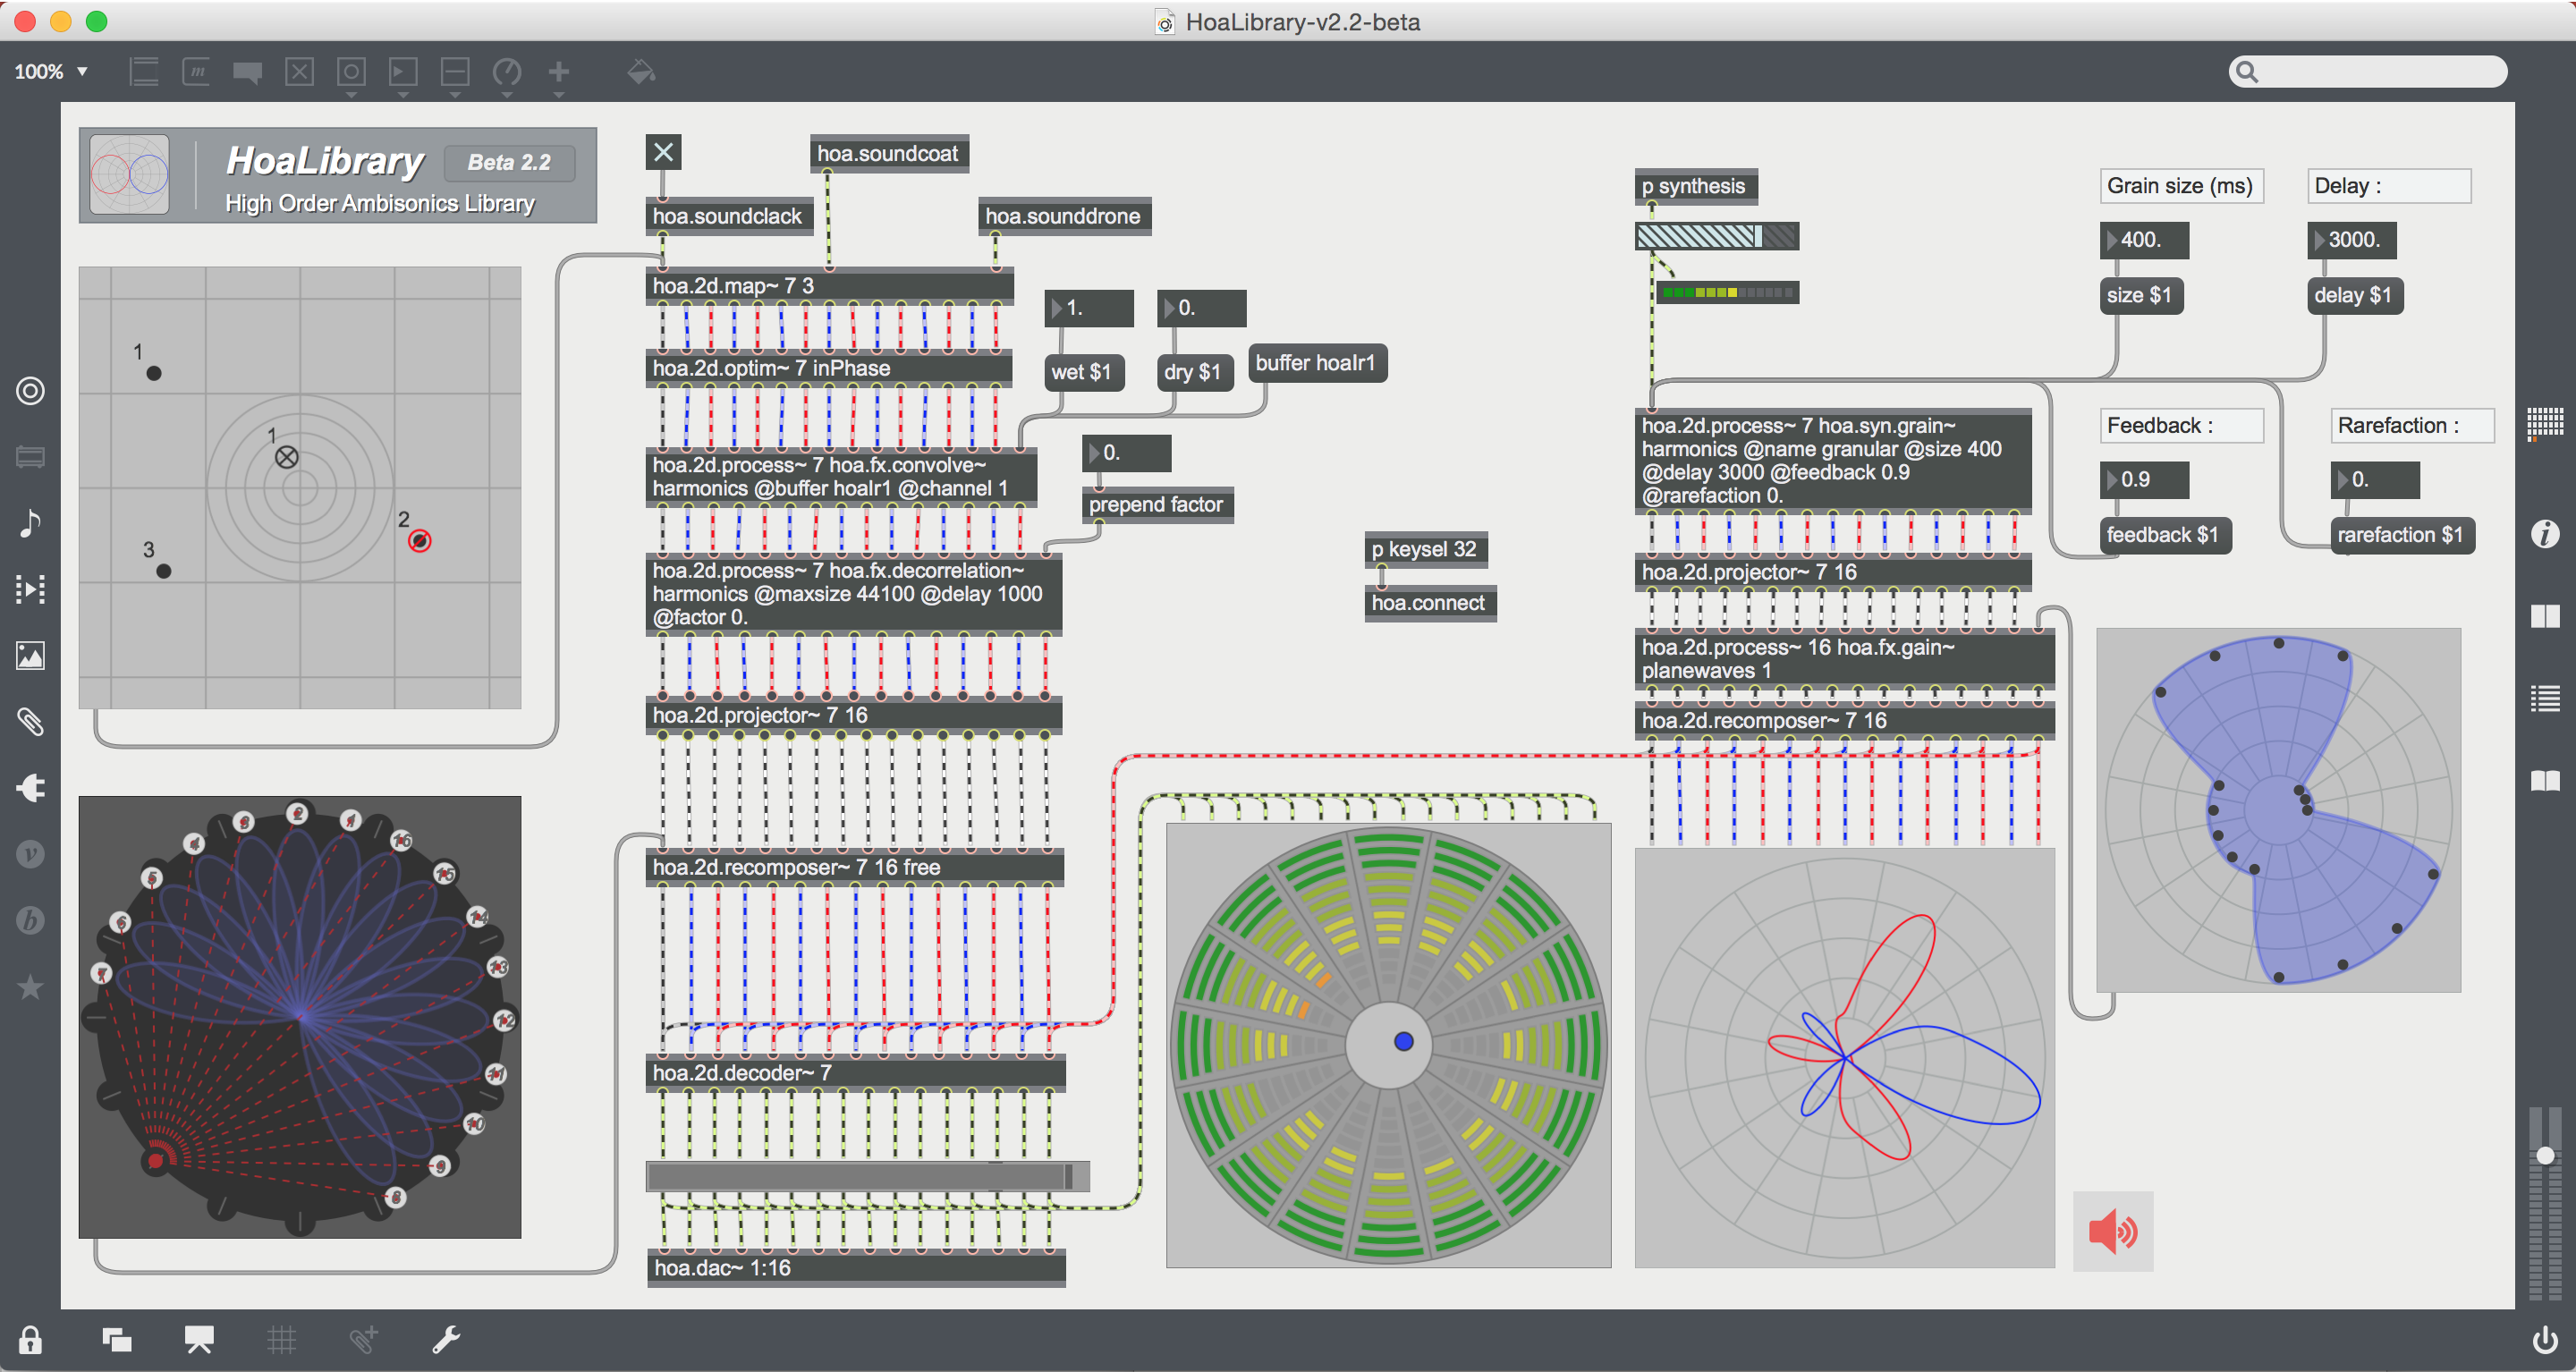
\includegraphics[scale=0.25]{images/hoalibrary.png}
    \caption{La bilbiothèque HOA.}
    \label{fig.hoalib}
\end{figure}

Utilisation dans la musique, ainsi que dans des applications de réalité augmentée.

Problème principal dans cadre musical : couplage fort entre l'écriture et le moyen de restitution. Par exemple il est souvent nécessaire d'ajuster les paramètres de spatialisation quand on change l'endroit ou se déroule une représentation. %TODO trouver source.
Par exemple, la bibliothèque HOA~\cite{colafrancesco_bibliotheque_2013} (fig.~\ref{fig.hoalib}) permet l'encodage et le décodage ambisonique ou binaural. Elle fournit en même temps des outils permettant de modifier et travailer la position des sons dans l'espace, et qui peuvent donc être utilisés à fin d'écriture.

Nous étudions aussi le cas de l'audio dans un cadre de systèmes interactifs : ce sont des systèmes soit très statiques comme dans un audio-guide, soit très dynamiques mais avec une boucle d'exécution simple.
Par exemple, il est possible d'apposer des couches audio dans un espace réel à l'aide de cartes pour faire des parcours\cite{lemordant_augmented_2010}. 


\subsubsection{Composition et écriture}
\begin{figure}[h]
    \centering
    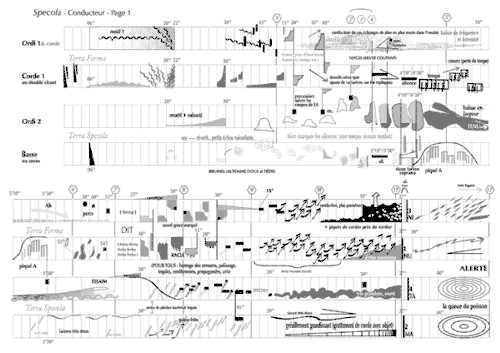
\includegraphics[scale=0.5]{images/specola.jpg}
    \caption{\textit{Specola} (LL de Mars) - une pièce acousmatique dont la partition est constituée de nombreux éléments graphiques spécialisés.}
    \label{fig.specola}
\end{figure}

Une présentation de l'état actuel de l'écriture spatiale en musique est donnée dans~\cite{fober_les_2015}. Notamment, la question de la notation dans le cadre de partitions impliquant des éléments spatiaux est abordé. % CITER PARTITIONS GRAPHIQUES.
Ces partitions peuvent être spatiales uniquement dans leur représentation, mais peuvent aussi indiquer des manières d'interpréter dans l'espace, notamment à l'aide de symboles spécialisés~\cite{ellberger_spatialization_2014}. Une taxinomie des possibilités de création dans l'espace en musiques électro-acoustiques est présentée par Bertrand Merlier dans~\cite{merlier_vocabulaire_2006}. Elle est étendue dans l'ouvrage \textit{Vocabulaire de l'espace en musique électro-acoustique\cite{merlier_vocabulaire_2006_book}}.

Des outils logiciels existent pour ces partitions -- ils sont souvent spécialisés. Par exemple, la bibliothèque \ac{ENP}\cite{kuuskankare_expressive_2006} permet de concevoir des partitions graphiques telles qu'en fig.~\ref{fig.specola} à l'aide d'un éditeur lui aussi graphique et d'un langage basé sur LISP.


Une des problématiques actuelles pour la représentation de l'écriture musicale est celle du geste, et de son lien avec la partition : comment notamment annoter le geste du musicien avec précision ? Et, inversement, comment à partir d'un geste créer un son correspondant ? Ces questions sont abordées dans la description de Soundstudio 4D\cite{sheridan_soundstudio_2004}, dans le cadre d'un système de conception de trajectoires pour spatialisation à l'aide d'interactions en trois dimensions.

Une autre question est l'association entre l'aspect graphique et le résultat. Ainsi, des outils tels que HoloEdit et HoloSpat permettent de travailler avec des trajectoires, mais sont extrêmement spécialisés pour des objets audio. C'est notamment du à la nécessité de composer en ayant conscience à chaque instant des fortes contraintes techniques du moyen de restitution de l'œuvre. Il serait intéressant d'utiliser ces trajectoires pour contrôler non pas des sources sonores mais des éléments dans des espaces de paramètres quelconques.

\begin{figure}[h]
    \centering
    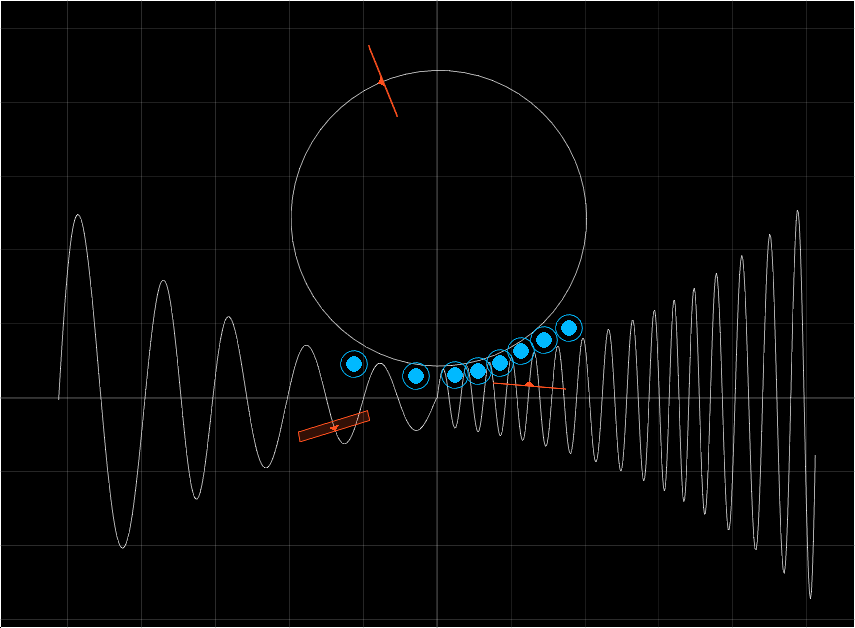
\includegraphics[scale=0.3]{images/iannix.png}
    \caption{Le logiciel IanniX.}
    \label{fig.iannix}
\end{figure}

Le logiciel IanniX\cite{jacquemin_iannix_2012} (fig.~\ref{fig.iannix}) dispose aussi de nombreuses possibilités d'écriture spatiale : les partitions sont des ensembles d'éléments graphiques définis paramétriquement ou bien à l'aide d'un langage de programmation dédié, que des curseurs vont parcourir. L'information de position de chaque curseur est envoyée en OSC, ce qui permet l'intégration à d'autres logiciels.

Une méthode d'écriture de la spatialisation par contraintes est proposée par Olivier Delerue avec le système MusicScpace\cite{delerue_spatialisation_2004}. Cela permet une approche déclarative à l'écriture de partition, en spécifiant des contraintes telles que <<~deux objets ne doivent jamais être à plus de deux mètres l'un de l'autre~>> ou bien <<~l'angle entre deux objets et l'auditeur doit être supérieur à 90 degrés~>>. Les objets peuvent être notamment des sources sonores. Une édition graphique de ces contraintes est proposée, et elles sont représentées en termes de cercles et de segments reliant les objets qu'elles contraignent.

Des données spatiales peuvent aussi être utilisées directement pour créer des mappings sonores. C'est le cas notamment de la bibliothèque Topos\cite{naveda_topos_2014}, qui permet de capter le mouvement de danseurs et d'en extraire des informations pouvant être utiles pour la conception de pièces de musique interactives. Une fois que le mouvement du danseur est capturé via un périphérique externe, il devient possible d'extraire des informations telles que le volume occupé par le danseur, sa vitesse, ou bien diverses mesures relatives à l'évolution de deux ou quatres points dans le temps, comme l'instabilité ou les collisions entre différentes parties du corps. Ces données peuvent ensuite être réutilisées dans Pure Data pour de la génération de musique.

Enfin, il convient de noter la richesse pour ce qui est des modes d'entrée et d'interaction. Par exemple, il existe plusieurs possibilités de composition musicale à l'aide de tables interactives comme la Reactable\cite{kaltenbranner_reactable:_2006} et différentes approches dérivées qui peuvent être spécifiquement axées sur la spatialisation du son\cite{sasamoto_controlling_2013}.

\subsubsection{Composition dans des environnements en 3D}
Une approche particulière est celle de l'immersion dans un monde virtuel en trois-dimensions pour la composition de musique. Cette approche est présentée par Michael Wozniewski dans~\cite{wozniewski_framework_2006}. Cela permet de définir et visualiser la propagation potentielle des ondes sonores dans un espace donné. De plus, en utilisant des méthodes de tracking de mouvement et des casques de réalité virtuelle, il est possible d'ouvrir de nombreuses possibilités d'interaction manuelle avec des objets virtuels. L'implémentation est faite en PureData.

D'autres possibilités d'utilisation d'environnement 3d à des fins d'écriture musicale sont suivies par Florent Berthaut avec le DRILE\cite{berthaut_drile:_2010}. Notamment, l'interaction spatiale est utilisée pour manipuler une hiérarchie plus aisément que via des interactions \ac{WIMP} traditionnelles.

Dans les deux cas, ce sont des approches orientées vers la manipulation d'objets.

\subsubsection{Acoustique virtuelle}
Il existe plusieurs méthodes pour simuler un environnement virtuel (comme par exemple dans un jeu vidéo) sur le plan acoustique, en tenant compte de la géométrie dans laquelle peut se trouver le joueur.

\begin{figure}[h]
    \centering
    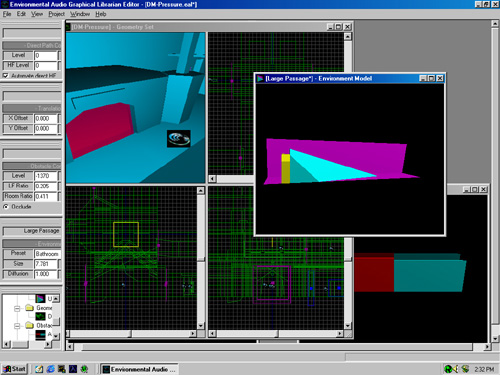
\includegraphics[scale=0.65]{images/eax.jpg}
    \caption{E.A.G.L.E., l'éditeur EAX.}
    \label{fig.eax}
\end{figure}

Les approches les plus simples utilisent simplement une atténuation linéaire entre la position du microphone virtuel, souvent appelé \textit{listener}, et les sources sonores qu'il peut y avoir. C'était le cas notamment pour certaines implémentations d'OpenAL\cite{hiebert_openal_2005}. Différents procédés, comme ceux proposés par la technologie EAX\cite{funkhouser_survey_2003} (fig.~\ref{fig.eax}), permettent d'ajouter une forme d'occlusion basique, ainsi que des effets de réverbération statique dans des endroits donnés pour enrichir l'impression d'espace. Des outils plus récents tels que FMOD et wWise s'intègrent notamment avec les moteurs de jeux pour pouvoir tirer parti directement des objets positionnés dans l'espace du moteur de jeu.

Cependant, il existe peu d'approches permettant d'être créatif par rapport aux possibilités qui sont offertes par l'outil informatique : notamment, les sources sont souvent ponctuelles alors que rien n'empêche de réfléchir à des sources planes ou volumétriques. 

Le rendu se fait généralement à l'aide de méthodes de lancer de rayon, inspirées des procédés utilisés en images de synthèse \cite{funkhouser_beam_1998,tsingos_fast_1998}.
Un procédé courant est maintenant d'utiliser les \ac{GPU} pour effectuer des calculs lourds mais facilement parallélisables\cite{rodriguez_performance_2014,cheng_design_2014,taylor_guided_2012}. Il est aussi possible de précalculer une fonction de convolution correspondant aux environnements virtuels que l'on veut parcourir, cependant cela demande des ressources en mémoire très importantes\cite{raghuvanshi_parametric_2014}.

\subsubsection{Restitution spatiale}
Il existe de nombreuses méthodes pour effectuer un rendu de son spatial. Certaines s'intéressent au rendu d'une "scène" spatiale donnée le mieux possible à l'aide d'un certain nombre de hauts-parleurs, tandis que d'autres visent la simulation d'une acoustique virtuelle comme nous l'avons vu précédemment. Comme pour HOA, les outils de création sont souvent fortement associés au système de rendu. La bibliothèque 3Dj\cite{perez-lopez_3dj_2015} pour Supercollider vise à séparer cela à l'aide d'une architecture modulaire séparant le mapping d'interface utilisateur, la gestion de scène spatiale, les comportements, les modèles physiques, l'export et le rendu via méthodes ambisoniques, HRTF\cite{noisternig_3d_2003}, \ac{VBAP}, \ac{DBAP} et \ac{WFS}.
La communication entre la gestion de la scène et le rendu se fait via le format standardisé SpatDIF\cite{peters_spatial_2013} par OSC. % TODO décrire plus loin

Une autre proposition d'architecture modulaire, par strates, est proposée par Nils Peters dans~\cite{peters_stratified_2009}.

Les différentes méthodes de spatialisation citées sont comparées via la capacité des auditeurs à situer la présence d'une source sonore dans l'espace dans~\cite{bates_comparative_2007}, et la précision de leur localisation.

L'intérêt de telles restitutions n'est pas seulement artistique : l'audio spatialisé peut être utilisé pour combler les déficiences visuelles, par exemple via un processus de sonification\cite{tang_assistive_2014}. Cela implique notamment une phase de reconnaissance d'objets, puis une phase de mapping d'un espace visuel défini hiérarchiquement vers un espace de sons qui permettra à la personne malvoyante de reconnaître des objets inertes via le son qui leur sera associé.

\subsection{Pratique liée à l'interaction}

% NOTE : faire partie qui différencie création via objets, création de mappings, création de trajectoires et qui compare les différentes approches que l'on a vu.
% NOTE : parler aussi de la gestion de l'environnement dans le son spatial (absorption de l'air, etc.)
% DIRE que certains modèles considèrent que les trajectoires sont un objet de premier plan mais pas d'autres. Trajectoires de premier plan signifie qu'une trajectoire peut notamment dépendre d'une autre et être déplacée elle aussi.
% TRAJECTOIRES : relatif / absolu ? 
% NOTE : dire qu'énormément de projets sont faits au cas-par-cas.
% NOTE : nécessité d'un méta-modèle de langage spatial & spatio-temporel ?
\subsubsection{Jeu vidéo}
\begin{figure}[h]
    \centering
    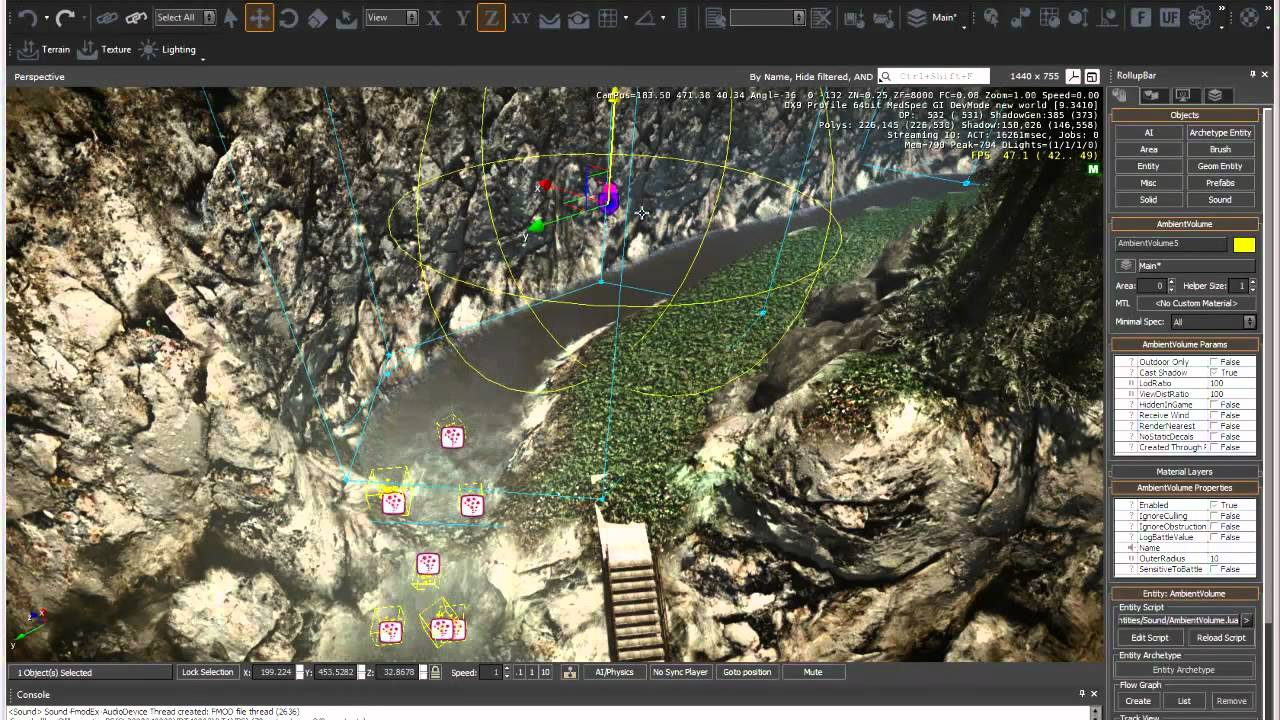
\includegraphics[scale=0.25]{images/cryengine.jpg}
    \caption{Positionnement de sources sonores dans le CryEngine}
    \label{fig.cryengine}
\end{figure}
La notion d'espace (et plus généralement, d'espace-temps) intervient à plusieurs échelles lors de la création de jeux vidéos. 
Elle est présente notamment à l'échelle du niveau de jeu, et décrit directement les interactions entre le personnage et son environnement, 
comme ce qu'il se passe lors d'une rencontre avec un ennemi ou un passage sur un objet bonus. 
Mais une notion plus large de narration spatio-temporelle va parfois sous-tendre le déroulement du jeu.
Liliana Salazar décrit dans sa thèse~\cite{salazar_modelisation_2004} différents modèles qui peuvent servir à décrire 
formellement un jeu vidéo; notamment des modèles basés sur les réseaux de Petri pour décrire les niveaux d'un jeu. 
Cela permet d'appréhender la complexité de telles œuvres : les jeux vidéos mêlent logique, temporalité, et spatialité.

Cécile le Prado s'intéresse plus particulièrement au lien entre les espaces visuels et sonores dans les jeux vidéos\cite{le_prado_ecriture_2013} par le biais de la cartographie.

Enfin, les moteurs de jeux généralistes tels que Unreal Engine, Unity, Unigine, Cry Engine, ont généralement des outils rudimentaires pour le positionnement du son (fig.~\ref{fig.cryengine}). Mais du fait de leur extensibilité, il existe une grande quantité d'outils implémentant divers algorithmes de spatialisation, comme par exemple 3Dception\footnote{\url{http://www.twobigears.com/3dception_unity.php}} (fig.~\ref{fig.3Dception}) ou IOSONO Proximity\footnote{\url{http://www.iosono-sound.com/game-audio}}. Cependant, il convient de noter que la partie qui est la plus travaillée durant la conception d'un jeu est généralement la partie graphique, et que le son spatialisé, malgré tout ce qu'il peut apporter, est traité comme un citoyen de seconde zone.

\begin{figure}[h]
    \centering
    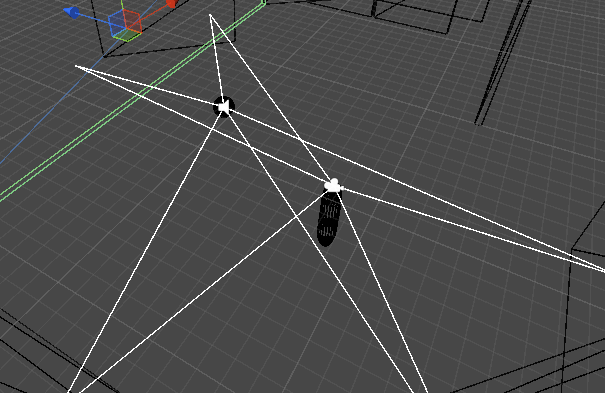
\includegraphics[scale=0.5]{images/3Dception.png}
    \caption{Réflexion du son dans 3Dception.}
    \label{fig.3Dception}
\end{figure}

De plus, dans de nombreux cas il n'y a que peu de travail sonore nécessaire : l'idée est de recréer un environnement réaliste, ce qui ne permet pas une marge de créativité énorme, mais demande plutôt des algorithmes précis.

\subsubsection{Interaction}
La majorité des outils que nous avons vu jusqu'à présent sont des outils de création qui fonctionnent peu ou prou avec le paradigme d'interface \ac{WIMP}, modulo des spécificités pour la création de jeux ou d'univers en 3D par exemple. Cette partie présente plus en avant les possibilités d'interaction qu'il peut exister dans le domaine spatial.

Nous distinguons deux aspects : la conception de contenu spatial est par essence une activité interactive que nous désirons étudier. 
Mais dans certains cas, on désire concevoir des applications offrant une part d'interactivité à l'utilisateur final, comme cela est le cas dans les bornes interactives par exemple. 
L'interaction étant souvent gestuelle, un modèle spécifique d'espace géré en temps réel mais conçu à l'avance devient alors nécessaire.
Ces deux aspects sont donc liés : une des thématiques qui nous intéresse est la conception d'outils de conceptions, notamment d'interaction. Il serait possible de parler de méta-conception.

Un état de l'art très complet pour l'interaction homme-machine dans un cadre de réalité mixte est présenté dans la thèse de René Chalon~\cite{chalon_realite_2004}. Outre une description des différents périphériques d'entrée-sortie disponibles à l'époque, sont présentés différents modèles adaptés à la gestion de l'interaction dans la conception d'une application en réalité mixte. Notamment, le modèle IRVO est introduit, et permet la séparation entre les objets réels, manipulés par l'utilisateur dans le monde physique, et ceux, virtuels qui sont uniquement présents dans la machine et représentés par projection. Une grande complexité réside dans l'interaction entre les deux espaces que sont le monde réel et virtuel, et le mapping d'informations de l'un à l'autre. Ces questions ont notamment été étudiées par Michel Beaudouin-Lafont avec la théorie de l'interaction instrumentale.

Un second état de l'art, plus récent et axé spécifiquement sur l'interaction qu'il peut y avoir avec les environnements 3D est présenté dans~\cite{jankowski_advances_2015}. Les méthodes d'interaction sont séparées entre celles qui ciblent la navigation dans un espace 3D, celles qui visent la sélection et manipulation de données, et celles qui permettent le contrôle des systèmes intermédiaires dans un environnement axé sur la 3D. 

Notamment, il existe des interfaces extrêmement spécifiques, qui peuvent souvent être utilisées à but artistique. Par exemple, le système BlowBrush\cite{shen_blowbrush:_2014} utilise un moulin à vent interactif pour peindre des feuilles sur un canevas virtuel.

Enfin, le développement des interfaces imaginaires\cite{gustafson_imaginary_2010}, qui superposent des informations virtuelles au monde réel sans pour autant avoir de forme visible, ouvre de nouvelles possibilités en terme de conception spatiale, car il devient possible de tricher quant à la localisation réelle des objets : dans le jeu de basket-ball imaginaire présenté, la position de la balle est par exemple régie par un système probabiliste et l'acquisition d'information par les joueurs se fait via le son.

\subsubsection{Muséographie}
Dans le cadre d'applications muséographiques, les informations spatiales sont au premier plan. Notamment, les points clefs sont : 
\begin{itemize}
    \item La conception d'interfaces utilisateur accessibles et adaptées à différentes classes d'age. 
    Michael Despina présente plusieurs faits intéressants, via une comparaison d'installations interactives dans~\cite{michael_comparative_2010}. Par exemple, pour une installation donnée, ce n'est pas parce qu'il y a un grand nombre de degrés de liberté en entrée ni que le contenu est en 3 dimensions que des enfants prennent du plaisir et ont envie de revenir participer à l'installation. C'est plutôt le type d'activité proposée qui va déterminer la qualité de l'expérience, peu importe le médium. De plus, l'auteur note une certaine réticence des jeunes enfants à approcher d'eux-même les installations basées sur un écran par opposition aux formats en table interactive, notamment due à de potentielles restrictions sur l'utilisation d'ordinateur à domicile.
    \item Des visualisations et univers graphiques et sonores spécifiques à chaque projet.
    \item Des modes d'interaction variés. Notamment, la place de l'interaction multi-touch, désormais très utilisée, est étudiée dans~\cite{kidd_multi-touch_2011}.
\end{itemize}

\begin{figure}[h]
    \centering
    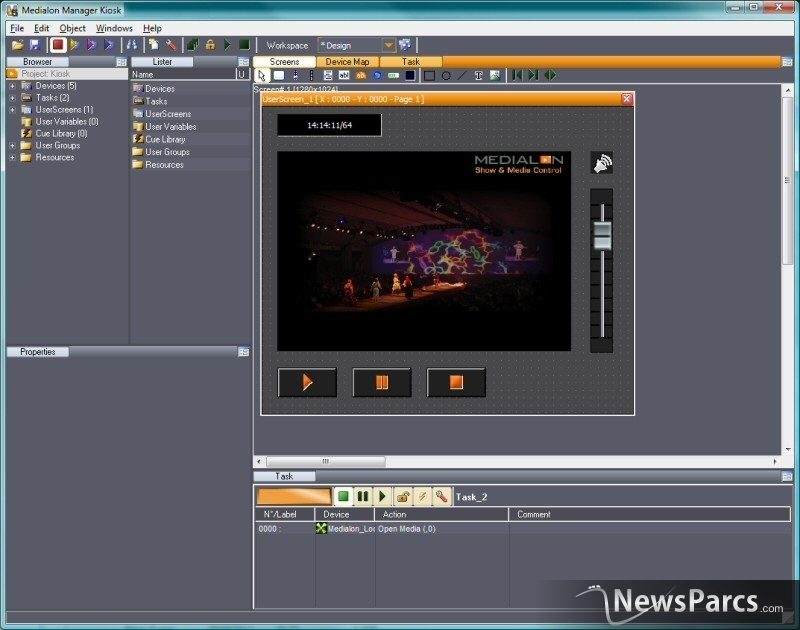
\includegraphics[scale=0.25]{images/medialon.jpg}
    \caption{Medialon KIOSK, un outil de conception de bornes interactives.}
    \label{fig.medialon}
\end{figure}
Le parc logiciel repose généralement sur des outils graphiques comme Adobe Flash, des bibliothèques spécialisées comme Processing ou OpenFrameworks, et des outils de conception génériques tels que Medialon (fig.~\ref{fig.medialon}).

Dans le cadre de parcours muséographiques et d'enrichissement du patrimoine culturel, il existe différentes approches qui visent à augmenter les œuvres et présentations. Par exemple, il est possible de sonifier des tableaux par rapport à différentes méthodes de segmentation, telles que des méthodes simples par clef de couleur. C'est le cas pour le logiciel SUM\cite{adhitya_composing_2012}.
Ce logiciel permet d'écrire de véritables partitions basées sur des tableaux, avec un système d'évolution dans le temps et en fonction du geste, qui permet de redécouvrir des tableaux sous un angle sonore.

Une autre approche pour l'enrichissement des visites de musées est présentée dans \cite{azough_modeet_2014}. L'approche vise à concevoir des paysages sonores à l'échelle d'une pièce ou même du musée entier, qui sont en lien avec le thème et se raffinent lorsqu'une œuvre en particulier est contemplée par les visiteurs. Un modèle (fig.~\ref{fig.visite.musee}) de visite de musée basé sur XML, permettant notamment de définir le degré de libertés accordé au participant est introduit. Il sépare, dans le cas de la scène sonore, les couches physiques et virtuelles qui ont déjà été abordées, ainsi que la couche sémantique.

\begin{figure}[h]
    \centering
    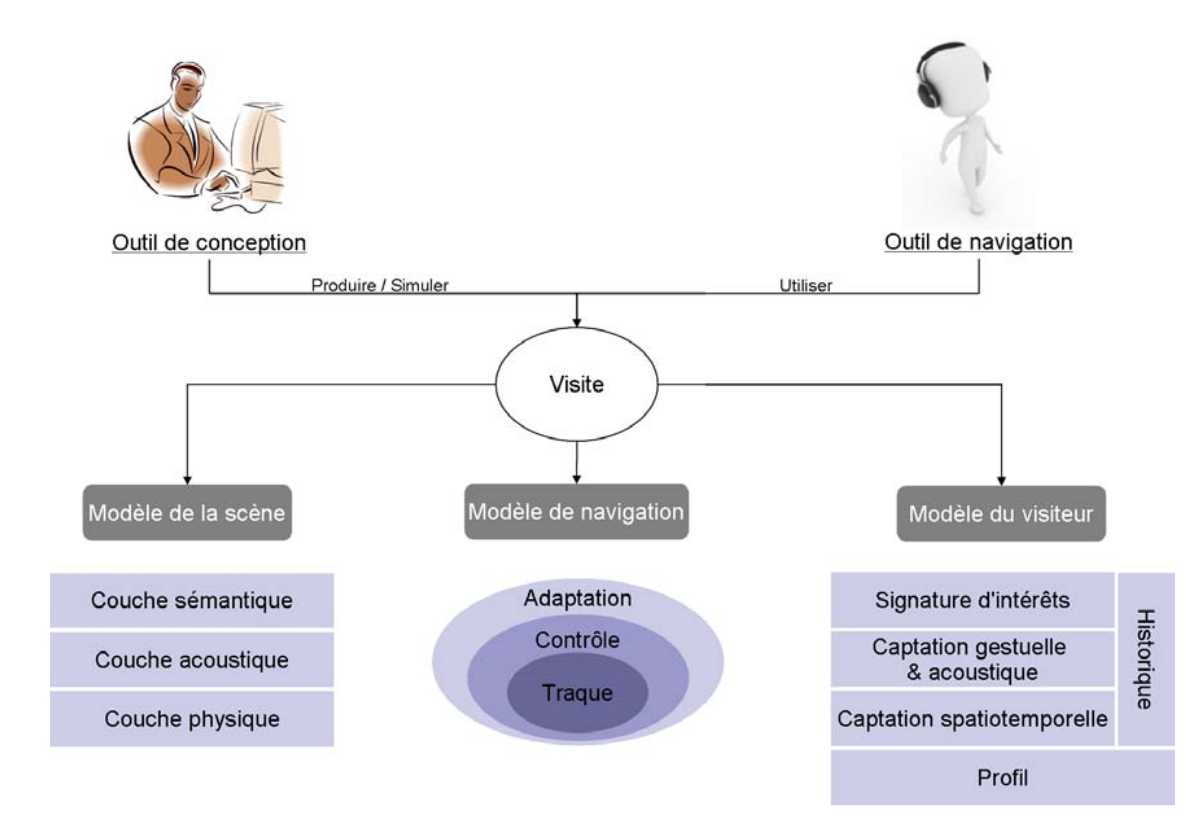
\includegraphics[scale=0.25]{images/modele_visite_musee.png}
    \caption{Modèle de structuration de visite de musée de Fatima Kaghat. Les trois modèles ont besoin d'outils appropriés de conception et de réaction adaptés à des données spatiales.}
    \label{fig.visite.musee}
\end{figure}

\subsubsection{Prévisualisation d'espaces}
Lors d'installations ou de spectacles complexes, une des grandes problématiques est celle de la prévisualisation, puis de la répétition.
Une possibilité est de concevoir des outils de storyboarding qui permettent de définir comment va se dérouler une pièce.

Cela pose de nombreuses questions quand au rôle de ces outils dans un cadre interactif. Par exemple, comment gérer le storyboarding de spectacles interactifs avec 
un certain nombre de libertés laissées aux acteurs ? Les problèmes les plus importants sont ceux de la synchronisation et de la remise dans un état donné.

Le framework ANSWER, présenté dans~\cite{jung_storyboarding_2010}, vise à fournir des outils pour le storyboarding de films, en partant 
du langage Director Notation permettant de spécifier le déroulement d'un film sur le plan conceptuel. Le problème est notamment
celui d'outil de spécification et conception permettant des esquisses de plans de caméra, de positions de décor et d'éclairage, etc.
L'approche utilisée est basée sur le système déclaratif orienté web X3D qui sera présenté en dernière partie de ce document.
D'autres langages, tels que TVML (en figure~\ref{fig.tvml}), sont aussi utilisés pour différents stages de la pipeline de production de contenu télévisuel et cinématographique.

\begin{figure}[h]
    \centering
    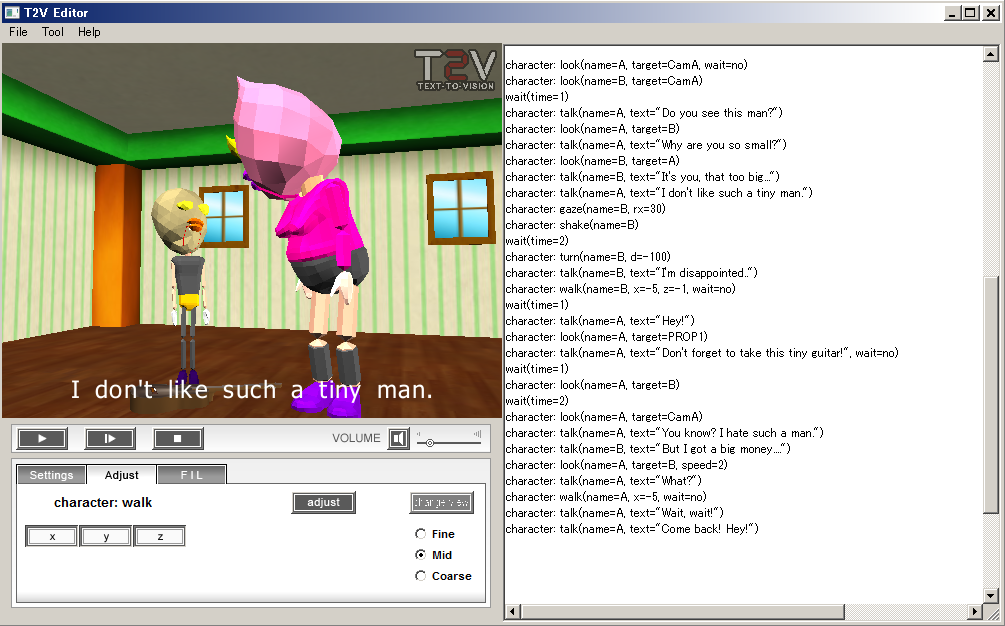
\includegraphics[scale=0.35]{images/tvml.png}
    \caption{Un exemple d'application de conception TVML, avec une partie prévisualisation et une partie langage. Ici, le langage est extrêmement spécialisé.}
    \label{fig.tvml}
\end{figure}

Un autre example de logiciel permettant l'écriture et la visualisation de scénographies est StageViz\cite{lee_stageviz:_2013}, développé en Corée du Sud.
L'intérêt de ce logiciel est son interopérabilité avec divers logiciels d'écriture, ce qui permet d'avoir un rendu graphique proche de 
ce que sera l'exécution réelle du spectacle à condition de fournir des modèles 3d adaptés et de fournir une brique d'intégration si un protocole spécifique est nécessaire. 
L'écriture se fait par successions d'états envoyés via des protocoles dédiés comme DMX.

\subsubsection{Robots}
L'écriture spatiale prend tout son sens lorsque l'on désire travailler avec des robots. De plus en plus d'artistes tentent de lancer des projets impliquant des robots musiciens, danseurs, ... et il est nécessaire de concevoir des outils adaptés. 
Notamment, les robots ont d'une part de fortes contraintes physiques dont il est nécessaire de tenir compte lors de l'écriture, et d'autre part, sont faillibles; il est nécessaire de concevoir des outils permettant d'adapter le spectacle lors d'une chute par exemple.

Un premier exemple est donné dans~\cite{lee_visualization_2013}. La question posée est surtout celle de la conception de robots adaptés à des spectacles:  un outil graphique est présenté, qui permet de concevoir facilement des robots par rapport à des modèles réels en combinant des moteurs virtuels en 3D. De plus, le robot virtuel réponds aux mêmes signaux que le robot réel. Il est alors possible de simuler la chorégraphie robotique sans avoir de problèmes de casse en cas de collision.

Cet outil est développé plus en avant dans~\cite{lee_virtual_2014} : un modèle permettant de calculer le couple appliqué par les moteurs du robot virtuel est rajouté au système, ce qui permet d'éviter d'autres problèmes au moment de l'écriture.
Pour cette étude, une comparaison probante a été menée entre deux robots réels et leurs avatars virtuels, en utilisant un système de motion capture.

\begin{figure}[h]
    \centering
    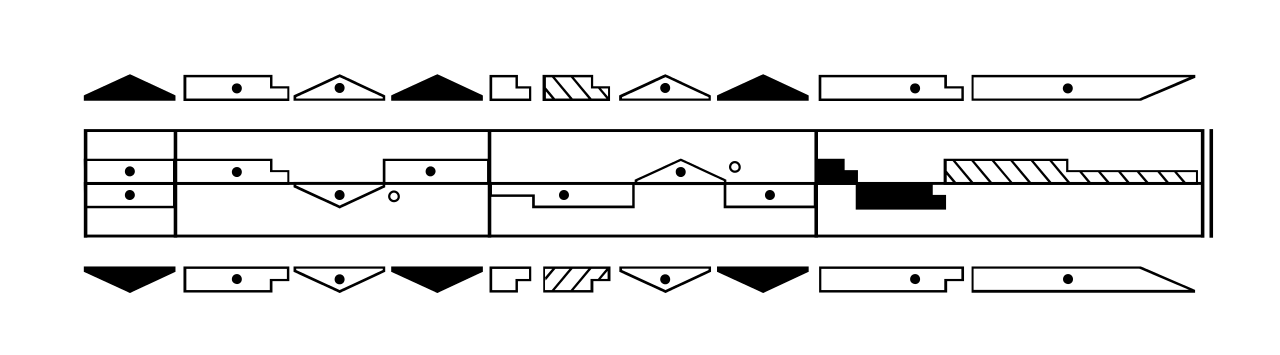
\includegraphics[scale=0.35]{images/Labanotation.png}
    \caption{Exemple de Labanotation pour la danse. Il est possible de spécifier la direction, l'intensité, la durée et la partie du corps correspondant à un mouvement.}
    \label{fig.labanotation}
\end{figure}

Il est aussi possible d'utiliser des méthodes de mapping pour laisser plus de liberté au robot. Ainsi, dans \cite{seo_autonomous_2013} un système de reconnaissance de musique générant des mouvements de danse en rythme est présenté. Cela part du constant que la plupart des chorégraphies pour robot ont actuellement besoin d'être programmées à la main, ce qui est particulièrement fastidieux. La chorégraphie est ici annotée à l'aide de Labanotation (fig.~\ref{fig.labanotation}), qui est une notation pour la danse, et reposant sur 12 mouvements basiques du corps humain. La forme des symboles rappelle la position du corps et des articulations.

Enfin, les dernières avancées technologiques permettent d'utiliser des drones en plus de robots traditionnels. Une utilisation intéressante est celle des Spaxels~\cite{hortner_spaxels_2012} : chaque drone devient une sorte de pixel spatial, qui porte une couleur et peut se déplacer comme il le désire dans un volume donné (fig.~\ref{fig.spaxels}).   
Un des problèmes majeurs lors de l'écriture d'une telle chorégraphie sera la gestion de l'inertie et des collisions : là encore, un outil de prévisualisation prenant en compte les lois physiques et les conditions que peuvent rencontrer les drones sera nécessaire.

\begin{figure}[h]
    \centering
    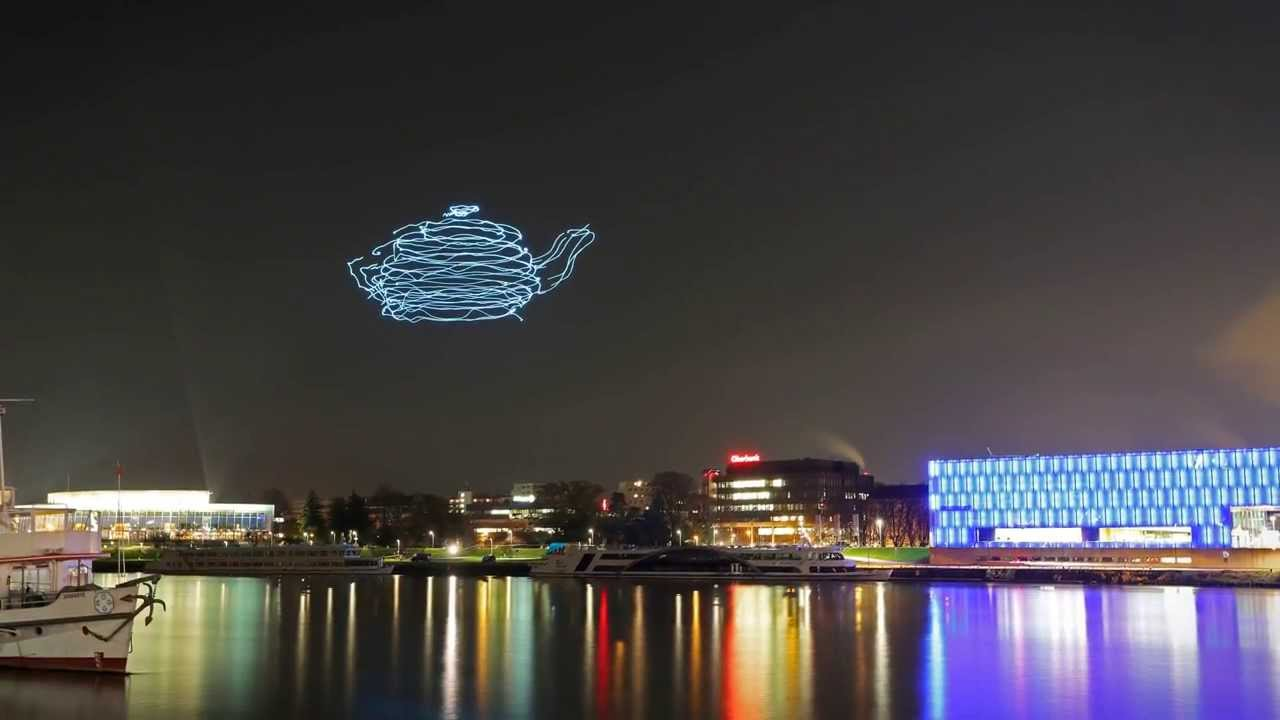
\includegraphics[scale=0.25]{images/spaxels.jpg}
    \caption{Des spaxels réalisent une forme à l'aide de trainées lumineuses.}
    \label{fig.spaxels}
\end{figure}

\newpage
\section{Outils de manipulation et d'écriture}
% TODO intro section

Jacob Beal présente dans~\cite{beal_spacetime_2015} les possibilités de gestion de l'espace-temps dans des applications à l'aide d'appareils connectés. Ces objets, comme les smartphones et smartwatches, étaient auparavant simplement connectés à un réseau, mais ont maintenant des informations de localisation et position, ainsi que de nombreux autres capteurs très précises avec lesquelles il est possible de concevoir des applications opérant sur de larges échelles géographiques. L'approche utilisée est de traiter l'ensemble des appareils connectés comme un champ, et de programmer des applications en utilisant les lois physiques qui régissent ces champs.

\subsection{Extraction de données}
Une possibilité couramment employée pour l'écriture est celle du mapping, c'est-à-dire que des données sont extraites d'un premier médium, transformées, puis appliquées à un second médium. Cela peut être, par exemple, la transformation d'un mouvement en image ou d'un son en un autre son.

À cet effet, il est utile d'avoir des métriques que l'on peut utiliser comme source de mapping. À titre d'exemple, Congcong Li présente dans~\cite{li_aesthetic_2009} 26 différentes métriques qui peuvent être extraites de tableaux et qui permettent de mesurer les qualités esthétiques, et par la suite de classifier les tableaux par style. La notion d'esthétique est empirique : dans ce travail, elle est basée sur une étude avec 42 participants et 100 tableaux; les participants devaient dire pour chaque tableau s'il était de bonne ou mauvaise qualité puis répondre à un questionnaire détaillé sur les facteurs de qualité perçus. Par la suite, cela a permise de chercher des métriques pouvant influencer ces aspects plus détaillés.
Des exemples de métriques extraites sont la clarté moyenne logarithmique, ou bien la forme des segments d'un tableau après segmentation algorithmique.

Il serait par la suite intéressant d'appliquer ces métriques en temps réel à des flux vidéos; cela fournirait un espace de paramètres importants avec lequel travailler. 

\subsection{Trajectoires et animation}
Une des problématiques les plus importantes est celle de l'écriture des trajectoires. Pour ce faire, il existe de nombreuses approches que nous séparons en deux parties : celles axées sur une entrée directe qui est ensuite analysée, par exemple avec un stylo électronique, et d'autres basées sur des méthodes mathématiques comme des équations paramétriques.

Rhonda\footnote{http://rhondaforever.com/} rentre dans la première approche. C'est un logiciel de dessin en trois dimensions à partir d'une entrée en deux dimensions et d'une source de rotation comme un gyroscope ou une souris adaptée. Il est utilisé dans Sonic Wire Sculptor et Ink Space, détaillé dans~\cite{rasmuson_flying_2013}. Une telle méthode d'entrée serait efficace pour définir des trajectoires spatiales car elle demande une interaction très simple.

\begin{figure}[h]
\begin{center}
\subfloat[Keyframes]{
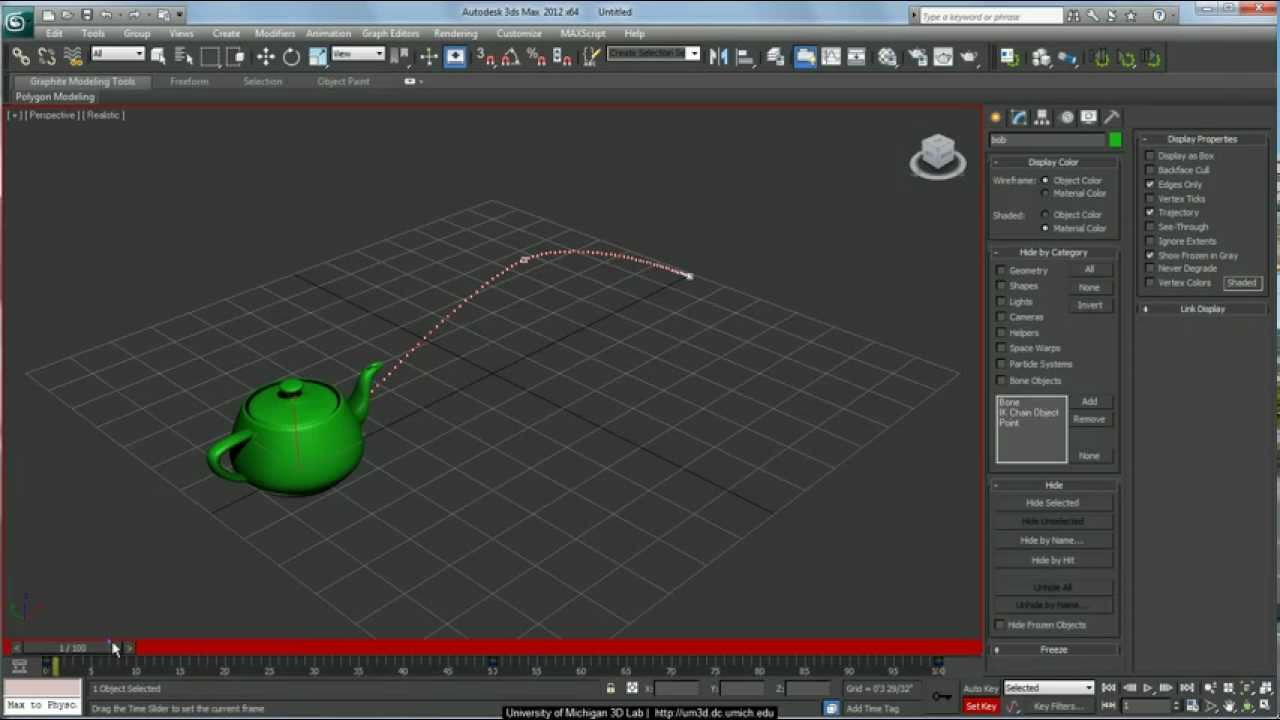
\includegraphics[scale=0.2]{images/3dsmax_keyframes.jpg}
\label{fig.sub.keyframe}
}

 \subfloat[Rotoscoping]{
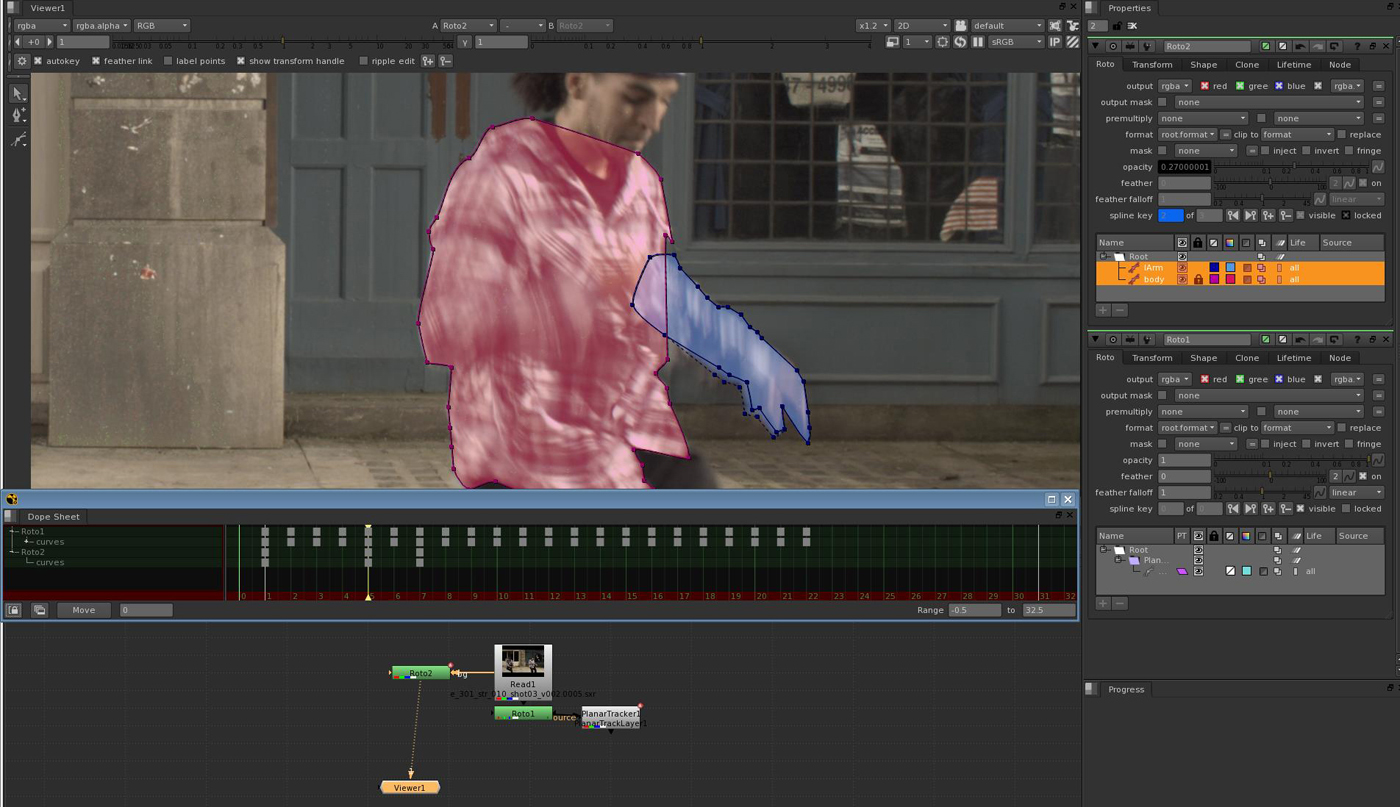
\includegraphics[scale=0.18]{images/rotoscoping.jpg}
\label{fig.sub.roto}
}
\caption{Modes d'animation standards : keyframes et rotoscoping}
\label{fig.animation}
\end{center}
\end{figure}
C'est en opposition avec les logiciels généralistes d'animation graphique, vectorielle ou vidéo. Les techniques les plus utilisées dans ce cas sont celles des keyframes et du rotoscoping (fig. \ref{fig.animation}).

La problématique principale en animation est de lier l'espace et le temps. Les méthodes par keyframes donnent priorité au temps, tandis que les méthodes par rotoscopie sont centrées sur des modifications d'espaces. De plus, dans les outils existants, le contrôle du flot du temps est généralement séparé de la création des données spatio-temporelles (les trajectoires). 

Une solution est proposée dans~\cite{santosa_direct_2013}, en utilisant un crayon pour contrôler le temps via les trajectoires lors de l'animation.

Une autre possibilité, implémentée dans Kitty\cite{kazi_kitty:_2014} repose sur la création de textures kinétiques : les textures, qui généralement ne sont que des informations de couleur, contiennent ici une information de déplacement. Plusieurs types de textures kinétiques sont présentés : des textures émettrices qui génèrent des objets, ainsi que des textures oscillantes qui animent un objet donné. Un graphe relationnel est ensuite utilisé pour définir les interactions qu'il peut y avoir entre les différentes entités de l'animation. Par exemple, cela permet de faire rebondir une balle lorsqu'elle <<~tombe~>> sur une table. Il est ainsi possible d'avoir des animations dynamiques et interactives qui peuvent répondre à une stimulation extérieur, après création (fig.~\ref{fig.kitty}).

\begin{figure}[h]
    \centering
    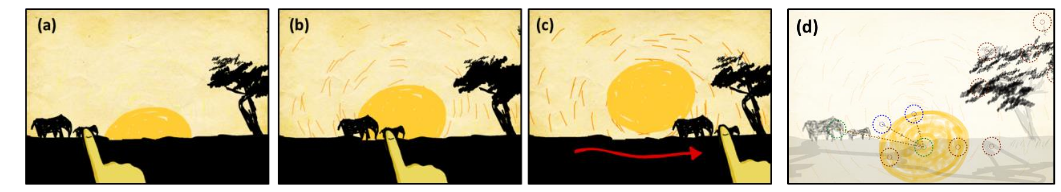
\includegraphics[scale=0.42]{images/kitty.png}
    \caption{Un exemple d'animation dynamique avec Kitty. Le soleil se lève lorsque l'éléphant est déplacé.}
    \label{fig.kitty}
\end{figure}

Une description interactive de trajectoires représentant des mouvements contraints par les lois physiques habituelles en 2D est explorée avec PhysInk\cite{scott_physink:_2013}. 
La cible est notamment l'enseignement de la physique et de la mécanique plane et le logiciel est sensé fonctionner comme un tableau blanc, mais qui possède une gestion des collisions réaliste. 
Dans ce système, l'utilisateur décrit un comportement en le dessinant.
 Les modifications faites sont gardées en mémoire : cela devrait permettre, à terme, d'effectuer des comparaisons entre plusieurs mouvements décrits dans un même document.

Enfin, la question de la représentation d'une animation se pose. 
En effet, il est souvent important pour l'auteur d'avoir non seulement l'état actuel mais aussi l'état passé et futur d'un élément lorsqu'il se positionne à un point $t$ dans le temps. 
Ce n'est pas problématique pour une trajectoire qui ne serait que fonction du temps, et donc qui peut être représentée comme une ligne dans un espace --- même s'il existe un problème de représentation évident d'un espace 3D sur un écran 2D, pour lequel des pistes sont apportées dans~\cite{cohen_interface_1999}.
En revanche, l'animation d'éléments graphiques ou bien dans plus d'une dimension, comme par exemple une animation au cours de laquelle un objet subirait un morphing, pose des problèmes de représentation. 
Une solution adaptée à la représentation des animations suite à capture de mouvement est présentée dans~\cite{casas_4d_2013}. 
Les logiciels d'animation standard se contentent généralement d'afficher les $n$ images précédentes et suivantes avec une opacité décroissante. 
Ces problèmes sont encore accrus dans le cas ou l'on aimerait prendre en compte l'interactivité : dans ce cas, il n'y a plus qu'une seule ligne de temps, mais un ensemble d'évolutions possibles pour les objets. 

\subsubsection{Trajectoires et espaces}
- État de l'art sur l'édition de courbes 3D en séparant en deux axes : le dispositif physique (entrée - sortie) et le langage d'interaction (création / édition de courbe, et manipulation de la caméra).
\cite{jacob_design_2014} % NOTE: état de l'art intéressant au début.


\subsubsection{Spatialisation du son}
Nous nous intéressons maintenant au cas précis de l'écriture de trajectoires pour le son. 
Ces trajectoires décrivent le déplacement d'objets sonores invisibles mais dont on est sensé pouvoir donner la position lorsqu'on écoute la pièce.

Une étude menée avec plusieurs compositeurs a permis de cibler certains des besoins 
qui sont exprimés lors de la pratique d'écriture de musique à l'aide de contraintes spatiales.
Cela est fait dans ce cas précis par le biais du logiciel Trajectoires\cite{favory_trajectoires:_2015} qui fonctionne sur dispositifs mobiles multitouch, 
et est implémenté avec des technologies web.

\cite{garcia_jeremie_processing_2015,garcia_towards_2015} % TODO bof : plutôt pour gestion du son

Un modèle plus complet d'espace en trois dimensions est fourni par COSM\cite{wakefield_cosm:_2011}.
Implémenté dans Max/MSP, il offre une grande richesse d'écriture.
En plus de lieux et de trajectoires, il est possible d'écrire l'interaction dans une certaine mesure, 
ainsi que la communication entre différents agents.
Une nouveauté est la possibilité de travailler avec des champs définis mathématiquements. 
Ces champs peuvent varier dans le temps et être sonifiés par la suite.

\begin{figure}[h]
    \centering
    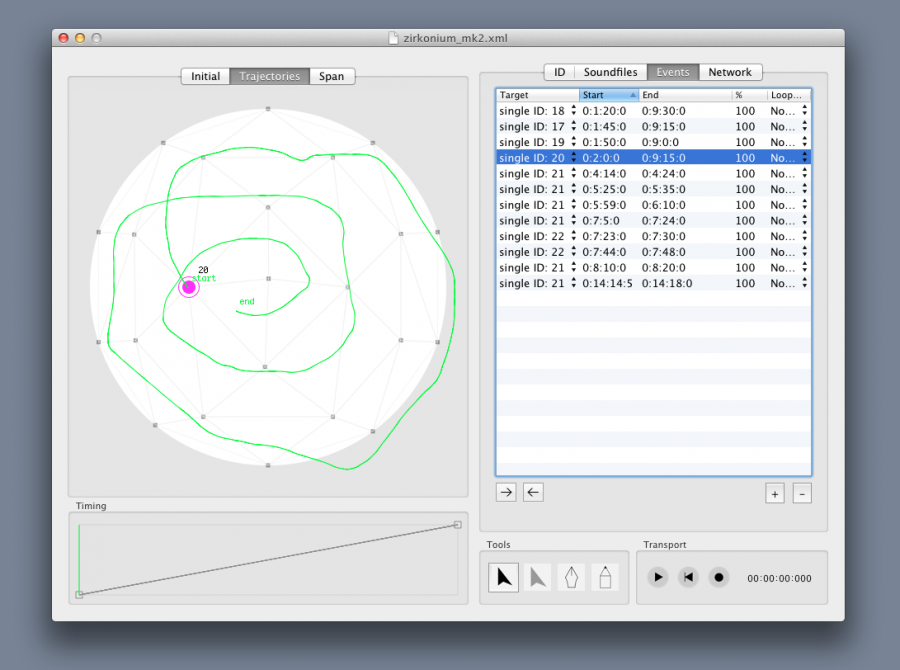
\includegraphics[scale=0.35]{images/zirkonium.png}
    \caption{Éditeur de trajectoires du Zirkonium Mk. 2.}
    \label{fig.zirkonium}
\end{figure}

Le Zirkonium, en fig.~\ref{fig.zirkonium} est un ensemble d'applications pour Apple OS X à l'origine conçues pour spatialiser le son du Klangdom, un lieu otpimisé pour la diffusion multi-canale du son. C'est un système logiciel basé sur une architecture client-serveur, et pourvur d'un éditeur de trajectoires spatiales pour le son qui permet notamment d'utiliser des courbes de Bézier pour l'écriture\cite{wagner_introducing_2014}. Les briques logicielles communiquent par OSC ce qui permet une certaine souplesse.

Un autre système de spatialisation, cette fois basé sur la réalité augmentée et utilisant la méthode \ac{WFS} est présenté dans~\cite{melchior_authoring_2005}. Notamment, une liste d'interactions possibles est présentée, ainsi que leur résultat dans le système. Il est notamment possible de diposer spatialement les sources sonores, d'ajuster des effets audio, et de simuler l'acoustique d'autres pièces en interagissant avec des objets dont la forme est concue pour avoir un lien avec les son auxquels ils se rapportent.

OpenMusic, avant d'être un système permettant spatialisation, est un outil très puissant de composition informatique. Basé sur la forme graphique du \textit{patcher}, à l'image de Max/MSP et PureData, il agit de manière entièrement hors-ligne. Le paradigme de programmation sous-jacent est fonctionnel (cela permet une conception simple du flot de données) et orienté objet.
Depuis quelques années, OpenMusic est doté d'outils pour la composition de musique avec des composantes spatiales\cite{bresson_spatial_2012}. Le modèle utilisé est une matrice joignant les sources sonores à des paramètres de spatialisation, qui vont évoluer dans le temps. 
Les trajectoires sont définies en coordonnées cartésiennes, et peuvent être dotées d'un tag temporel qui permet de faire le lien avec l'écoulement du temps dans le morceau. Cela se rapport à la notion de keyframe vue précédemment. Les données spatiales ont la particularité de pouvoir être utilisées aussi lors de la synthèse des sons, et non pas seulement comme un filtre qui serait appliqué après génération comme c'est le cas dans la majorité des autres approches.

- bibliothèque de spatialisation en C++, permettant la traduction entre différents formats de données spatiales audio.
\cite{wozniewski_spatosc:_2012}

\subsubsection{Manipulation tangible}
- Manipulation tangible de courbes à l'aide d'un périphérique spécifique, ShapeTape, qui est déformable 
et permet d'obtenir informatiquement sa torsion en 32 points pour reconstruire la courbe de manière virtuelle en 3D : 
\cite{grossman_interface_2003}

\subsection{Autres approches}
- Génération d'espace à partir de description textuelle.
\cite{andriamarozakaniaina_du_2012} 

- Conception de mappings en trois dimensions dans Max/MSP. 
Mappings de régions de l'espace via interpolation :
 le mapping a lieu entre N dimensions de contrôle et M dimensions sonores.
\cite{van_nort_lom_2006}

 - Zones ? logiciels de 3d paramétrique, etc. 
 % TODO parler des approches standard par keyframes, etc. au début

\newpage
\section{Modélisation}
Il existe trois grandes familles de modèles utilisés pour la représentation de données spatiales : 
\begin{itemize}
\item Les modèles quantitatifs : ce sont simplement les modèles basés sur des coordonnées cartésiennes. 
\item Les modèles qualitatifs : ils s'intéressent aux relations entre objets dans l'espace. Notamment, des formes de logique spécialisées sur l'espace existent et seront présentées plus en avant. Un ouvrage de référence sur ce sujet est le \textit{Handbook of Knowledge Representation}\cite{porter_handbook_2008}.
\item Les modèles spécialisés : souvent issus du génie logiciel, ils visent à répondre à un problème précis, comme la localisation géographique à une certaine précision ou des systèmes en réalité virtuelle et augmentée.
\end{itemize}

- Construction d'une ontologie du raisonnement spatio-temporel basé sur la notion de réalité. Séparation entre évènements \textit{continuants} et \textit{occurents}. Ces composants de l'ontologie générale présentée servent de point de vue sur la réalité et peut ou non interagir avec les autres. La persistence des continuants se fait par l'existence de parties temporelles successives; le temps est une dimension de spécification des occurents mais pas des continuants.
\cite{grenon_formal_2003}

- possibilités probabilistes

- Modèle d'automates spatio-temporels adaptés à la gestion de systèmes de transports % TODO bof....
\cite{zhang_timed_2014}

- Modèle d'espace pour l'interaction en réalité virtuelle. Apporte les notions de moyen, d'aura, d'awareness..
\cite{benford_spatial_1993}

- Modélisation fonctionnelle des animations via un DSL dédié en haskell. Présupposé : toute animation a un début, un milieu et une fin. Combinaison d'animations.
\cite{matlage_every_2011}

\subsection{Modèles de données}
Ontologie pour le web. Application aux \ac{GIS}.
- OWL : \cite{mefteh_approche_2013}.

- X3DOM :langage déclaratif intégré au DOM HTML/CSS\cite{jankowski_declarative_2013}. Par opposition à WebGL qui est impératif.

- Adaptés à l'audio
. SpatDIF et compagnie \cite{peters_spatial_2013}\cite{kendall_towards_2008}
. \cite{kondoz_object-based_2014}

- Généralistes
- Programmation fonctionnelle réactive; là aussi, un DSL dédié en Haskell qui utilise les Arrow.
\cite{hudak_arrows_2003}

Approches langage : (pour reconnaissance : \cite{spranger_recruitment_2011}\cite{spranger_emergent_2012}, )

- Modèles qualitatifs : \cite{chen_survey_2015}, \cite{bhatt_geospatial_2014}, \cite{schlieder_qualitative_1996,dorr_qualitative_2014}. Spatio-temporel : \cite{hazarika_qualitative_2012}. \cite{clementini_global_1997}.

- Trajectoires : via équations paramétriques.

- Voxels : \cite{kaufman_volume_1993}

- Quadtrees : \cite{eppstein_skip_2008}
\subsection{Problèmes géométriques et calculatoires}
- citer bibliothèques utiles.
\printbibliography
\end{document}